\chapter{Event Reconstruction \& Simulation} \label{chap-EventReconstruction&Simulation}

Monte Carlo (MC) simulations are an essential part of current particle physics analyses and are used to mimic physical processes that correspond to those which are observed within the LHC, and other such experiments. Analysts compare findings in data to simulation in order to extract signal processes, and also to perform statistical analysis on results obtained. It is of the utmost importance that the simulated events must be as accurate as physically possible in order to mimic real life processes and perform a scientifically accurate analysis. Will talk about methods for generating events, including the different MC generators and tunes used in the evaluation of theoretical uncertainties, and interpretation in terms of the CMS detector in the first section of this chapter.

Roughly speaking, we can divide the different steps of event reconstruction into three separate processes. The first of which records basic information, such as hits within the pixel detectors of the inner tracking system, and calorimeter energy clusters, for `low level' objects in each sub-detector. The information is then passed to the PF algorithm (Section \ref{subsec-PFAlgorithm}) which uses information from all the sub-detectors in order to reconstruct events much more accurately. Finally, the events are refined by other complex statistic and mathematical techniques and used to reconstruct higher level objects, such as jets and MET. The second part of chapter will focus on the PF process \cite{CMS-PAS-PFT-09-001, CMS-PAS-PFT-10-001} as mentioned above.

\section{Event Reconstruction} \label{sec-EventReconstruction}

\begin{figure} [p!] 
\begin{center}
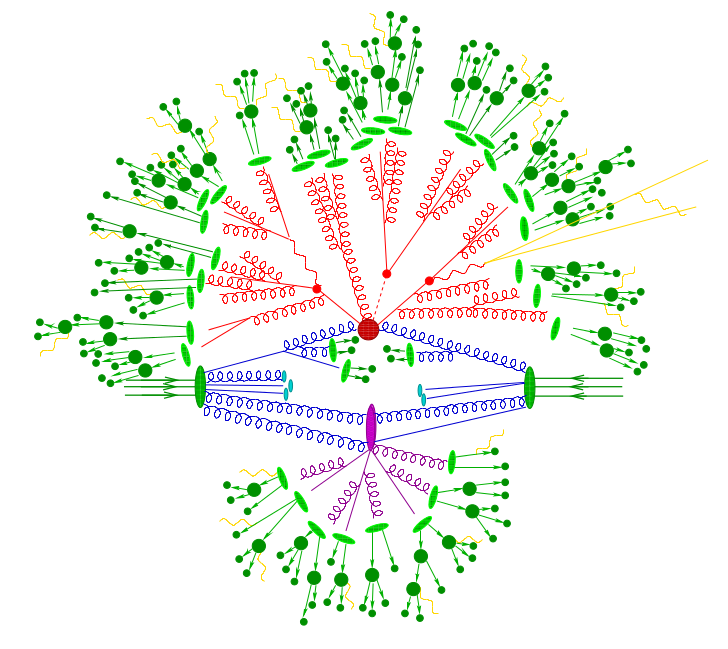
\includegraphics[scale=0.55]{Figures/HadronCollisionProcess.png}
\end{center}
\caption{Graphic visualisation of a hadron collision process where two partons come in from the right and the left, represented by the directional arrows. Two gluons (purple) form the hard scattering interaction (red circle). This section of the process depicts the matrix element calculation. In the hard scattering interaction prompt decays and parton showers then take place as represented by the smaller red circles. Finally, the hadronisation process begins (green circles). We also observe collinear gluon emissions as well as underlying event particles stemming from a softer collision with other partons in the hadrons. This is represented by the purple circle. \cite{HadronCollisionProcess}.}
\label{fig-HadronCollisionProcess}
\end{figure}

\section{Computing}

\subsection{Event Data Model}

Physically, an event is the result of the hard scattering process created when the LHC collides two bunches of protons together. We cannot know the full properties of an interaction without processing the data, and this is where the Event Data Model (EDM) is derived. The information about the event is measured as energy deposits, clusters, and tracks in each sub-detector of the CMS experiment that is read out by a series a processing electronics. When it comes to reconstructing the data and performing statistical analysis, we read in an event as a C++ object storing the raw data. These objects are presented to a user stored as ROOT files \cite{Brun199781}. There are three different data formats that data is stored as, each of which contains a different level of precision for describing events. The three levels are as described below.

\begin{description}
	\item[RAW] file formats contain very primal information about the data, including the L1 and HLT decisions. At this stage events have a size of roughly 1.5 MB. 
	\item[RECO] is the next step in the formatting of data by reconstructing events obtained from the RAW format with pattern recognition and compression algorithms. This includes reconstructed detector hits, calorimeter clusters, and reconstructed physics objects such as electrons, jets etc. The typical event size at this level is around 250 kB.
	\item[AOD] (Analysis Oriented Data) is created by filtering (performing quality checks etc) the RECO data from the reconstructed detector-level objects, where the higher level physics objects are calculated. The size of the events is reduced to $\sim50$ kB.	
\end{description}

Almost all physics analysis groups use the RECO and AOD data formats. All data used in this analysis uses the AOD data format, where event sizes are reduced by filtering the RECO data, as can be seen in Table \ref{tab-MCSamples}. The objects are delivered in the data files as C++ objects, which are then transformed into vectors or plain basic types. By selecting on the physics objects that are central to our analysis, we can further reduce the event size to $\sim$3 kB, which we call the ``skimming", thus reducing the run time of an analysis. The processing of RECO and AOD formats for analysis begins with taking the data and using a specifically designed framework to process a set of ``nTuples'' for each physics process, and categorising them into classes, such as objects. The benefit of constructing such ``nTuples'' lies in the reduction of processing time by allowing the analysis to be run locally, rather than re-processing the full dataset in AOD, RECO, or RAW from each time. 

\subsection{Analysis Software} \label{subsec-AnalysisSoftware}

Analysis is usually performed within a computing environment specific to an experiment. CMS provides an extensive software framework, CMSSW \cite{CMSSW}, that provides users with a large range of algorithms to create, handle, and analyse data. $\CMSSW$ is fundamental in regards to MC simulation, detector calibration and alignment, and then for the reconstruction of data and analysis thereof. The framework is a modular structure that combines a single configurable executable (cmsRun) with a number of plugin modules containing event processing algorithms. $\CMSSW$ is continuously being updated to keep up-to-date with new analysis techniques and processes. The versions of $\CMSSW$ used in this analysis are listed below:

\begin{itemize}
	\item CMSSW\_5\_3\_9 for the analysis of $t\bar{t}+\gamma$.
	\item CMSSW\_5\_2\_10\_nTuple for the ntuple processing for the $t\bar{t}+\gamma$ analysis.
\end{itemize} 

The framework used is of a modular design, similar to $\CMSSW$. The code is split into different modules designed to model the data at various stages of processing. We essentially design four modules to carry out the reading-in of the data, transferring it into a readable C++ format, selecting and implementing cuts on our events, and outputting the information in the form of a histogram in order to statistically analyse the data, as described below. 

\begin{itemize}
	\item Reader files that translate plain data types stored in ROOT files into C++ objects. 
	\item Reconstruction objects process the output of the readers in the form of real objects, such as leptons and quarks.
	\item Selections are written for each decay channel in an analysis to select on objects that exist in the final state of an event.
	\item Analysers are used to create histograms of different variables at various stages of selection, implement scale factors, and add weights to samples. 
\end{itemize}

\section{Simulation of the CMS detector}

The simulation of the CMS detector is an incredibly complex task and very time consuming to run such a simulation. In order to perform such a procedure $\GEANTfour$ \cite{GEANT4} is used to simulate the geometry of the whole detector, divided into sub-detectors, and track the particles as they pass through the different materials. Implemented within the $\CMSSW$ framework are two packages that perform detector simulation, Full Simulation (FullSim) \cite{FullSim} and Fast Simulation (FastSim, previously named FAMOS) \cite{1742-6596-513-2-022012}.  
In the FastSim package physical processes are described in detail, such as the electromagnetic and hadronic interactions, energy deposits, and electronic detector responses. The FastSim package is designed with a much lower level of detail incorporated and reduces the computational time by 3 orders of magnitude. This allows analysts to carry out custom MC productions within a reasonable time. A comparison between the two packages is shown in Figure \ref{fig-FullSim}. 

\begin{figure} 
\begin{center}
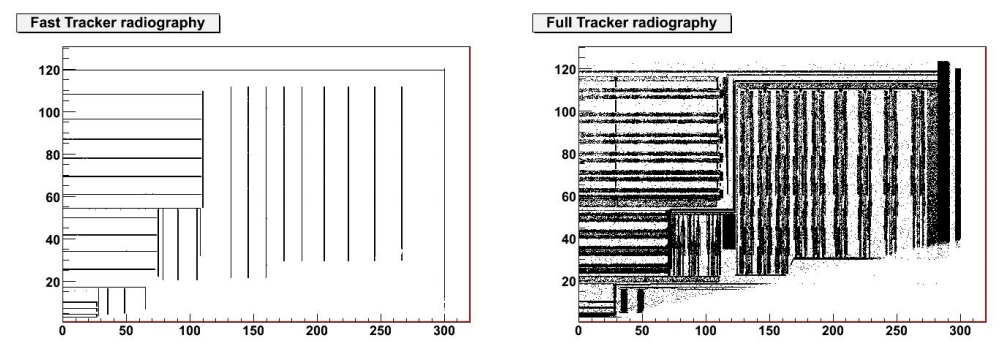
\includegraphics[width=\textwidth]{Figures/FullSim.png}
\end{center}
\caption{A radiography of a quarter of the simulated tracker geometry in the (a) fast and (b) full simulation \cite{1742-6596-513-2-022012}. The data points are from the vertices of converted photons, whereby we have a much larger of simulated events in the fastsim.}
\label{fig-FullSim}
\end{figure}

\section{Monte Carlo Simulation}

\subsection{Monte Carlo event generators} \label{subsec-MCEventGenerators}

MC generators are programs that simulate the properties of particles such that results can be compared to those obtained from data in order to perform a statistical analysis and verify findings. CMS uses many event generators in order to simulate specific physics processes that are of interest. Hard scattering processes are simulated via matrix element calculation and then parton showering is subsequently added. In order to convolute the two procedures a matching is implemented. Finally, hadronisation is then modelled as the showered partons form colourless bound states with other partons. MC event generators produce a list of all particles/partons that are created in an event along with their kinematic properties, such as p$_T$, and includes production of underlying events (UE) and additional primary vertex interactions from pile-up (PU). Underlying events are classified as any source of interaction produced that does not originate from the initial hard scattering process, such as initial and final state radiation (ISR and FSR), and remnants from the beam. We define PU as any other interaction produced from the same bunch crossing as our hard scattering. Bunch crossings can contain up to 20 different interactions, that is to say 20 different primary vertices are observed. Figure \ref{fig-HadronCollisionProcess} shows the hard scattering collision process as produced by MC event generators. 

In the analysis presented in this thesis each physical process was simulated by different MC event generators, such as $\WHIZARD$ $\MADGRAPH$ $\PYTHIA$ $\MCATNLO$ $\POWHEG$. The MC event generators which are used in this analysis, as previously mentioned, are described in more detail below. Generators are usually combined by interfacing with another generator in order to optimise for each simulation step described in Section \ref{sec-EventReconstruction}. An example of this can be seen within the main background sample for this analysis, the $t\bar{t}$ sample, which is generated using both $\MADGRAPH$ and $\PYTHIA$.   

\begin{description}

	\item[\WHIZARD] \cite{WHIZARD} is a LO event generator designed to calculate multi-particle scattering cross-sections efficiently and simulated event samples. Tree-level matrix elements are automatically generated for arbitrary partonic processes, in particular the MSSM is supported including an interface to the SUSY Les Houches Accord (LHA) input format. It is also possible to interface matrix elements from alternative processes, such as loop corrections. WHIZARD uses a multi-channel method for phase space integration, meaning that it involves simultaneous use of multiple phase space parametrisations corresponding to dominant Feynman diagrams, and is able to calculate numerically stable signal and background cross-sections and also generate unweighted event samples with a reasonable efficiency for final state events containing up to 6 or more particles, meaning that it generates uniformly distributed events each contributing the same event weight to the sample. The polarisation of initial and final states is treated in the same manner, and quark and lepton flavours are automatically summed over where needed. For hadron collider physics studies, the standard LHAPDF library is incorporated. For fragmentation and hadronisation of the final states, $\PYTHIA$ and $\HERWIG$ interfaces are provided, both of which follow the Les Houches Accord. 

	\item[\MADGRAPH] \cite{MADGRAPH5} is a leading order multi-purpose matrix-element MC generator. Similar to the WHIZARD generator, $\MADGRAPH$ automatically generates matrix elements for scattering processes with up to 6 and above final state particles. The matching of matrix elements to parton showers is performed following the MLM prescription \cite{Hoche:2006ph} only if a parton-jet pair satisfies a predefined $\Delta R$ requirement, and if none, or more than one jets, are found then the event is rejected. There is also a certain p$_T$ threshold for partons that they must pass in order to be considered for matching.

	\item[\PYTHIA] \cite{1126-6708-2006-05-026} is a widely used tool in the particle physics community. It is used for the generation of events within high-energy collisions, and it does so by utilising a complex set of physics models to process the evolution of a 2-body (or more) scattering to a complex multi-particle final state. The generator contains a library of hard processes, models for parton showers for initial and final states, matching among hard processes and parton showers, multi-parton interactions, beam remnants, string fragmentation and particle decays.  

	\item[\MCATNLO] \cite{1126-6708-2002-06-029} provides a method for matching next-to-leading order (NLO) calculations of QCD processes with a particle shower from simulation in MC. $\MCATNLO$ improves on many aspects with respect to a LO generator, such as $\PYTHIA$. Aspects such as the total exclusive rates are accurate to NLO, hard emissions are treated as in NLO computations with soft/collinear emissions handled by MC, and matching between hard and soft emission regions is smooth. This provides an advantage for heavy flavour physics, such as top quark production. A small amount of events with negative weights are generated, however the process of unweighting is possible with a reasonable efficiency. 

	\item[\POWHEG] \cite{1126-6708-2007-11-070} (Positive Weight Hardest Emission Generator) is a NLO event generator similar to $\MCATNLO$ described above. The difference between the two arises in the basic idea behind $\POWHEG$, whereby it generates the hardest radiation first before passing the event to any shower generator to perform subsequent, softer radiation. Thus, as it does not depend on any parton shower program in particular, the output of $\POWHEG$ can be easily interfaced with any shower generator capable of handling the given user process. Another feature of $\POWHEG$ is that events can be created with positive (constant) weight.  


\end{description}	

\section{Simulated samples for the $t\bar{t}+\gamma$ analysis}

As previously mentioned, different MC samples are simulated using different event generators for various physical processes. Table \ref{tab-MCSamples} provides all the different MC sample datasets used in the $t\bar{t}+\gamma$ analysis along with their respective cross-sections and number of processed events in each sample. This section will focus on background samples where generation of the signal $t\bar{t}+\gamma$ sample can be seen in Section \ref{sec-mcsim} It can be seen that the main background to this analysis, TTJets ($t\bar{t}$), is was generated using the $\MADGRAPH$5 event generator and interfaced with the $\TAUOLA$ generator. $\TAUOLA$ is a MC event generator designed specifically for the modelling of tau lepton decays. The samples are then passed to $\PYTHIA$6 for parton showering and hadronisation as described in Section \ref{subsec-MCEventGenerators}. Each $t\bar{t}$ decay process, fully-leptonic, semi-leptonic, and fully hadronic is treated individually and generated as three independent samples. The advantages of treating the decay modes separately are that no scale factor has to be implemented in order to account for the different branching ratios of each decay channel and it is also more convenient to observe the $t\bar{t}+\gamma$ content in each channel separately.

Similarly, both Drell-Yan samples, W+Jets, $W+\gamma$, $Z+\gamma$, and diboson background samples are also simulated in the same fashion as the TTJets samples. Single top events are simulated in a slightly different fashion, whereby they are generated by the $\POWHEG$ generator, also described in Section \ref{subsec-MCEventGenerators}. Again, the events are then passed to $\PYTHIA$6 to model parton showering and hadronisation. Single top samples are also split into different decay modes: tW, s-channel, t-channel. Top quarks and anti-top quark processes are treated separately and simulated in different samples.

\begin{sidewaystable} 
\begin{center}
\resizebox{\textwidth}{!}{ 

\begin{tabular}{|l|c|c|c|} %|l| p{12.5cm} |c|p{2cm}|
\hline
	\textbf{Process} & \textbf{Dataset} & \textbf{$\sigma$ (pb)} & \textbf{Number of events} \\
\hline
	$t\bar{t}+\gamma (2\to5)$ & /LHE2EDM\_WHIZARD\_2to5\_ttA/htholen-FULLSIM\_STEP2\_WHIZARD\_2to5\_ttA-da43ae45efb6a7c35e17aad82de2e2cd/USER & 1.8 & 1074860 \\
	$t\bar{t}+\gamma (2\to7)$ & /TTGamma\_TuneZ2star\_8TeV-madgraph-tauola/Summer12\_DR53X-PU\_RD1\_START53\_V7N-v1/AODSIM & 1.8 & 916500\\ 
\hline	
	$t\bar{t}(Leptonic)$ & /TTJets\_FullLeptMGDecays\_8TeV-madgraph/Summer12\_DR53X-PU\_S10\_START53\_V7A-v2/AODSIM & 245.8 & 12119013\\
	$t\bar{t}(Hadronic)$ & /TTJets\_HadronicMGDecays\_8TeV-madgraph/Summer12\_DR53X-PU\_S10\_START53\_V7A\_ext-v1/AODSIM & 245.8 & 31223821\\
	$t\bar{t}(Semileptonic)$ & /TTJets\_SemiLeptMGDecays\_8TeV-madgraph/Summer12\_DR53X-PU\_S10\_START53\_V7A\_ext-v1/AODSIM & 245.8 & 25424818\\
	$t\bar{t}(Inclusive)$ & /TTJets\_MassiveBinDECAY\_TuneZ2star\_8TeV-madgraph-tauola/Summer12\_DR53X-PU\_S10\_START53\_V7C-v1/AODSIM & 245.8 & 6923652\\
\hline	
	Drell-Yann, $10 < m\_{ll} < 50$ & /DYJetsToLL\_M-10To50\_TuneZ2Star\_8TeV-madgraph/Summer12\_DR53X-PU\_S10\_START53\_V7A-v1/AODSIM & 11050.0 & 37835275\\
	Drell-Yann, $m\_{ll} > 50$ & /DYJetsToLL\_M-50\_TuneZ2Star\_8TeV-madgraph-tarball/Summer12\_DR53X-PU\_S10\_START53\_V7A-v1/AODSIM & 3350.0 & 30459503\\
\hline	
	$Z+\gamma$ & /ZGToLLG\_8TeV-madgraph/Summer12\_DR53X-PU\_RD1\_START53\_V7N-v1/AODSIM & 159.12 & 6588161 \\
\hline	
	Single Top tW & /T\_tW-channel-DR\_TuneZ2star\_8TeV-powheg-tauola/Summer12\_DR53X-PU\_S10\_START53\_V7A-v1/AODSIM & 11.1 & 497658 \\
	Single TopBar tW $\bar{t}$ & /Tbar\_tW-channel-DR\_TuneZ2star\_8TeV-powheg-tauola/Summer12\_DR53X-PU\_S10\_START53\_V7A-v1/AODSIM & 11.1 & 493460 \\
	Single Top t & /T\_t-channel\_TuneZ2star\_8TeV-powheg-tauola/Summer12\_DR53X-PU\_S10\_START53\_V7A-v3/AODSIM & 56.4 & 99876 \\
	Single TopBar t & /Tbar\_t-channel\_TuneZ2star\_8TeV-powheg-tauola/Summer12\_DR53X-PU\_S10\_START53\_V7A-v1/AODSIM & 30.7 & 1935072 \\
	Single Top s & /T\_s-channel\_TuneZ2star\_8TeV-powheg-tauola/Summer12\_DR53X-PU\_S10\_START53\_V7A-v1/AODSIM & 3.79 & 259961 \\
	Single TopBar s & /Tbar\_s-channel\_TuneZ2star\_8TeV-powheg-tauola/Summer12\_DR53X-PU\_S10\_START53\_V7A-v1/AODSIM  & 1.76 & 139974 \\
\hline	
	W+Jets & /WJetsToLNu\_TuneZ2Star\_8TeV-madgraph-tarball/Summer12\_DR53X-PU\_S10\_START53\_V7A-v2/AODSIM & 36257.2 & 57709905 \\
\hline	
	$W+\gamma$ & /WGToLNuG\_TuneZ2star\_8TeV-madgraph-tauola/Summer12\_DR53X-PU\_S10\_START53\_V7A-v1/AODSIM & 553.92 & 4802358 \\
\hline	
	Diboson WW & /WW\_TuneZ2star\_8TeV\_pythia6\_tauola/Summer12\_DR53X-PU\_S10\_START53\_V7A-v1/AODSIM & 56.0 & 10000431\\
	Diboson WZ & /WZ\_TuneZ2star\_8TeV\_pythia6\_tauola/Summer12\_DR53X-PU\_S10\_START53\_V7A-v1/AODSIM & 33.6 & 10000283\\
	Diboson ZZ & /ZZ\_TuneZ2star\_8TeV\_pythia6\_tauola/Summer12\_DR53X-PU\_S10\_START53\_V7A-v1/AODSIM & 8.2 & 9799908\\
\hline	
\end{tabular}
}
\end{center}
\caption{Dataset information for signal and background MC samples.}
\label{tab-MCSamples}
\end{sidewaystable}


\section{Simulation of the $t\bar{t}+\gamma$ Signal Sample} \label{sec-mcsim}

Three different techniques were used to define the $t\bar{t}+\gamma$ signal process. The concepts are illustrated in Figure \ref{fig-MatrixElementCalculation} and shows the final state of the process using each technique \cite{heinerthesis}. The parton distribution function CTEQ6L1 \cite{Pumplin:2002vw} is interfaced to $\WHIZARD$ via LHAPDF \cite{Whalley:2005nh}. The process utilises variable renormalisation and factorisation scales. This is such that, event by event, the two are set to $172.5 \GeV$ (m$_t$) plus the E$_T$ of the generated photon. Upon varying the scale of each, we arrive at a systematic uncertainty of $^{+7.0}_{-8.3}\%$, as shown in Chapter \ref{chap-SystematicUncertainties}. Initial and final state radiation is taken into account, as well as hadronisation, and is simulated using \PYTHIA6 \cite{Sjostrand:2006za}, $\TAUOLA$ and $\PHOTOS$ \cite{Was:2006my} as preconfigured in CMSSW. We use the same configuration as for the top-pair sample.

Restrictions on the final state particles have been set, named generation cuts, such that a proper integral is retained when calculating matrix elements. As a method to cope with infra-red divergences, soft gluon emissions, a minimum energy or momentum is required. We treat collinear divergences (collinear parton splitting) by introducing a minimum distance in the $\eta - \phi$ plane. These cuts likely will not affect the measurement due to the cuts within selection being tighter than generator levels cuts. The different generation cuts are described in brief below:

\begin{description}
\item[2 $\to$ 3] At this level only quantum mechanical interferences from initial state radiation are considered. The CPU time required in for tree level processes is moderate.

\item[2 $\to$ 5] In this case, the decay of the top quark is included and thus photons that have radiated from a W boson or a b-quark, as well as interference effects between the two, must be taken into account. This is a significant process, as we must expect photons stemming from a W or b to contribute significantly to our signal. Photons that are radiated from the W are considered negligible, because the W decay products are highly boosted in top-quark events giving rise to, mostly, collinear emissions. 

\item[2 $\to$ 7] In this scenario we consider photon radiation and interference from all decay products. CPU time is much more intensive in this case due to the many more Feynman diagrams to be computed.                                                                            

\begin{figure} 
\begin{center}
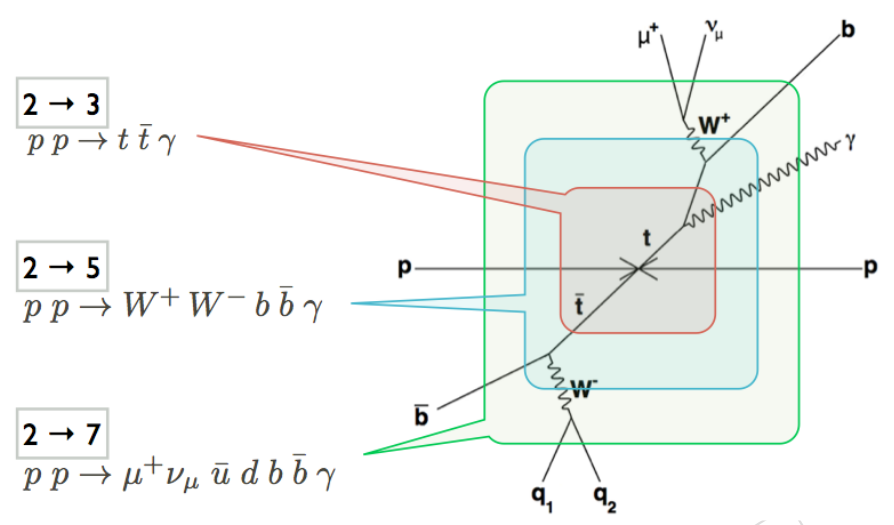
\includegraphics[width=\textwidth]{Figures/MatrixElementCalculation.png}
\end{center}
\caption{Process generation. The red, blue, and green boxes depict the matrix element calculation. Background processes with the same final state are included as well \cite{heinerthesis}.}
\label{fig-MatrixElementCalculation}
\end{figure}
                               

\end{description}

Originally, this analysis used the $2 \to 5$ technique with initial generator level cuts of $E_T > 20$ GeV and $\Delta R(\gamma, b/\bar{b}) > 0.1$ using WHIZARD \cite{WHIZARD}, which is a leading order (LO) event generator. The variable factorisation and renormalisation scales are set to $m_{top} + E_T(\gamma)$, and a scale variation uncertainty of 8\% has been applied to the WHIZARD $t\bar{t}+\gamma$ cross-section result, which gives $1.8 \pm 0.5$ pb as the SM expectation for the signal process, where the scale variation uncertainty, and uncertainty on the k-factor (the ratio between the NLO and LO cross sections as a function of some observable) are added in quadrature. 


\subsection{Official $t\bar{t}+\gamma$ $2 \to 7$ sample production}

The final version of the analysis uses the factorised $2 \to 7$ process for the simulation of the $t\bar{t}+\gamma$ signal sample. Instead of computing one single matrix element for the complete $t\bar{t}+\gamma$ process, we factorise the process into individual processes and calculate the matrix element for each sub-process. The major restriction on the calculation of the matrix element lies in the computational time, such that using a factorised matrix element method vastly reduces the computation time to calculate the matrix element. The matrix element is divided in the following manner:

\begin{align}
pp \to t\bar{t}+\gamma, \quad t \to bxx', \quad \bar{t} \to \bar{b}xx' \\
pp \to t\bar{t}, \quad t \to bxx'\gamma, \quad \bar{t} \to \bar{b}xx' \\
pp \to t\bar{t}, \quad t \to bxx', \quad \bar{t} \to \bar{b}xx'\gamma 
\end{align}

where $x = u,d,s,c,\bar{u},\bar{d},\bar{s},\bar{c}, e^{\pm}, \mu^{\pm}, \tau^{\pm}, \nu_{e,\mu,\tau}, \bar{\nu}_{e,\mu,\tau}$.

In order to verify the factorisation method, we generated a sample using WHIZARD with the full, un-factorised, $2 \to 7$ matrix element generation process, which we then compared to a sample simulated in WHIZARD using the factorised matrix element method. The results of this comparison can be seen in Figure \ref{fig-WHIZARDfullvsfactorised}, where we see a good agreement in the shapes of observables. We observe small fluctuations between bins within the full $2 \to 7$ sample, which we attribute to the number of events. We can therefore verify that the method can be used as a good approximation of the full $2 \to 7$ process.

Upon validation of the factorisation method for the full process, we observe the method to be a good compromise between accuracy and computational time. A comparison is then conducted between the $\MADGRAPH$ and WHIZARD event generators using the full $2 \to 7$ process. Within the WHIZARD framework, we are unable to compute the three factorised processes at the same time, and must therefore generate the individual processes separately and later combine them, whereby scaling is taken into account. 

For both generators, the original $pp \to t\bar{t}+\gamma$ process and the decay of the top quarks are distinct processes. The $\MADGRAPH$ framework handles both processes internally, however we must simulate the two must be handled individually in the WHIZARD framework and an extra set of kinematic cuts must be implemented, as shown below.

\begin{itemize}
	\item $p_T(\gamma) > 1$ GeV
	\item $\Delta R (\gamma, X) > 0.1$
\end{itemize}

These cuts are required to be softer than the final generator cuts, due to the dilution of kinematics by resolution effects at the value of the cuts. This is such that if the value of cuts used for decays is too close to the final generator cuts, resolution effects may be modelled incorrectly. When calculating the cross-section, WHIZARD does not take the final generator cuts into consideration. They are simply used to select events which are then written to the output file. The cross-section must be re-weighted when taking individual efficiencies into account, leading to the simulation taking more time than it would with the final generator cuts included, where a vast amount of generated events are rejected by the tighter cuts.

It must be noted that for simplicity, in the comparison we only select semi-leptonic events in the muon channel. However, for the full sample we incorporate all decay channels for the $2 \to 7$ process in order to be inclusive as possible since the sample will be an official CMS sample. 

\begin{figure} 
\begin{center}
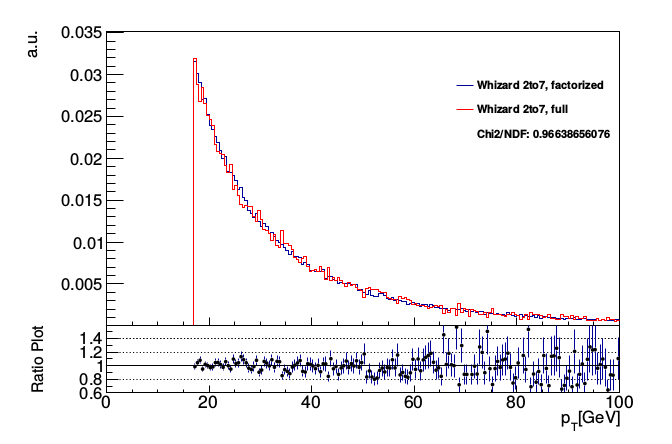
\includegraphics[width=0.9\textwidth]{Figures/WHIZARDfullvsfactorisedPT.png} \\
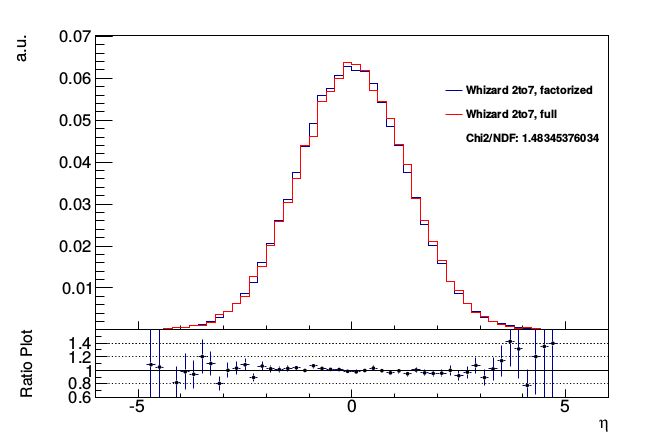
\includegraphics[width=0.9\textwidth]{Figures/WHIZARDfullvsfactorisedEta.png} \\
\end{center}
\caption{Comparison between the full and the factorised $2 \to 7$ process using samples generated with WHIZARD. All distributions are normalised to unity. \cite{ttgammasimulation}}
\label{fig-WHIZARDfullvsfactorised}
\end{figure}  

We calculate the cross-sections to be 

\begin{equation}
\WHIZARD : \sigma_{t\bar{t}+\gamma} = 1408 \xspace \text{fb}, \quad \MADGRAPH : \sigma_{t\bar{t}+\gamma} = 1227.1 \pm 0.4 \xspace \text{fb}
\end{equation}

for each event generator, respectively. We note that there is no associated error with the WHIZARD cross-section, this is due to the cross-section calculated with this event generator not taking the final cuts on the decay products into account. The final cross-section is calculated from the remaining number of events. Additionally, the branching ratios for the top decays are not included within the cross-section calculation, as additional calculations are required by the user. This is more of a feature in channels where a photon is required. 

The calculation steps, described previously, are estimated individually and the uncertainty on each usually contributes to the overall uncertainty by propagating them onto the final value. However, this is not calculated in this analysis, because the cross-sections are used to compare the event generators. Thus, an exact calculation of the errors is not necessary, and a NLO cross-section is used in the analysis which renders the differences inconsequential. The difference of 12.9\% observed between the two generators is thus within the expected range of deviation. 

A comparison between the two event generators for the factorised $2 \to 7$ process, for three key variables, can be seen in Figure \ref{fig-WHIZARDvsMADGRAPH}. We observe a good agreement between the two event generators except for small discrepancies in the angle between the photon and b quark at low values of $\Delta R (\gamma, b)$. We regard this discrepancy as irrelevant to our analysis due to the manner in which jets and isolation is handled in a proton-proton collider experiment such as CMS. Another explanation could lie within the normalisation process of the WHIZARD sample, and could affect the shapes of the distributions.

\begin{figure} 
\begin{center}
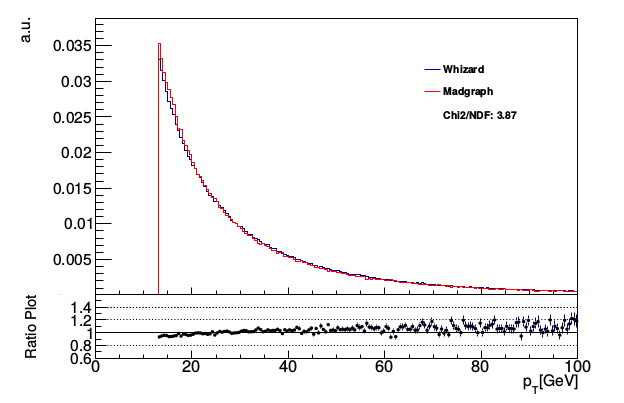
\includegraphics[width=0.8\textwidth]{Figures/WHIZARDvsMADGRAPHPT.png} \\
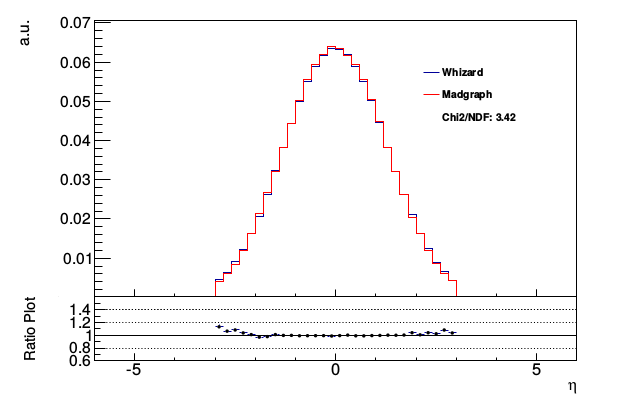
\includegraphics[width=0.8\textwidth]{Figures/WHIZARDvsMADGRAPHEta.png} \\
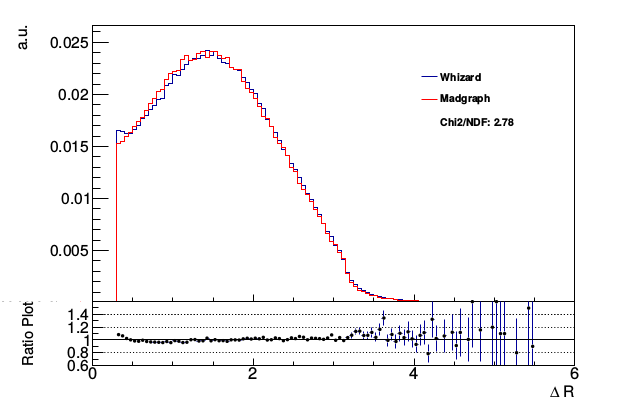
\includegraphics[width=0.8\textwidth]{Figures/WHIZARDvsMADGRAPHDR.png} \\
\end{center}
\caption{Comparison between the $\MADGRAPH$ and WHIZARD generators for the factorized $2 \to 7$ process. All distributions are normalized to unity. \cite{ttgammasimulation}}
\label{fig-WHIZARDvsMADGRAPH}
\end{figure}  

The cuts used in the generation of the \MADGRAPH MC sample are as shown below.

\begin{itemize}
	\item $p_T (\gamma) > 13 \GeV$
	\item $|\eta(\gamma)| < 3.0$
	\item $\Delta R (\gamma, all) > 0.3$, where ``all" refers to any other generator level particle
	\item $p_T (jet) > 15 \GeV$
	\item $p_T (b) > 20 \GeV$
	\item $|\eta (b)| < 5.0$
	\item $|\eta (jet)| < 5.0$
	\item $| \eta (lepton)| < 3.0$
	\item $\Delta R (jet, jet) > 0.5$
	\item $\Delta R (jet, lepton) > 0.5$
\end{itemize}

There is no cut on lepton transverse momentum, but there are cuts on the momenta of quarks (jets). This makes the ratio of hadronic and leptonic W decays generated with these cuts differ from W branching ratio without any cuts.

\section{Physics Object Reconstruction} \label{sec-ParticleObjectReconstruction}

The CMS experiment employs a complex algorithmic technique, Particle Flow (PF) \cite{CMS-PAS-PFT-09-001}, as part of a chain of reconstruction tools to reconstruct the full topology of events produced by collisions using information from each sub-detector. PF uses the information obtained from lower-level object reconstruction including tracking and clustering of energy deposits within each sub-detector. The primary goal of PF is to determine the object type, momentum, and energy for all objects within a singular event. Such objects include electrons, muons,  charged hadrons, neutral hadrons, and photons. This information is then used to reconstruct higher-level objects, such as jets and MET.

\subsection{Charged Particle Tracking} \label{subsec-ChargedParticleTracking}

The tracking of charged particles begins with the reconstruction of tracks in the inner detector system. As the charged particles traverse the detector they deposit energy which we call hits, an iterative tracking algorithm then inputs the information from a number of hits in order to reconstruct tracks of individual particles \cite{1748-0221-9-10-P10009}. By reconstructing the particle tracks we have access to information about the particle, such as the momentum before any effects from the magnet, and the impact parameter (IP), the distance of closest approach to this point used in later reconstruction. 

Around two thirds of the particles than constitute a jet are charged particles, therefore if we are able to accurately reconstruct the tracks of charged particles in the detector, and the accuracy for correctly reconstructing a jet increases greatly. As all objects are reconstructed using the PF algorithm, which uses tracker information to fit tracks before reconstructing higher-level objects (Section \ref{sec-HigherLevelObjects}) we see that information gleaned from tracker hits are vital for physics analysis. Several properties of tracks from the inner detector system contribute to its importance in reconstructing tracks, such as the $p_T$ resolution which, for charged hadrons with a $p_T$ of $\mathcal{O}(10^2) \GeV$, is significantly better than in the calorimeter systems.

One of the key parameters in object reconstruction is the track efficiency, the number of real tracks found over the number that incorrectly reconstructed or originate from a different source (`fake tracks'). Therefore, a high tracking efficiency is required in order to use the PF algorithm to it's full potential, and thus an iterative algorithm for tracking was designed \cite{1748-0221-9-10-P10009}. The tracking algorithm can be broken down into roughly 5 processes, which are described below:

\begin{description}
	\item[Local Reconstruction] records signals in the silicon strips and pixels, converts them into `digis' and then groups them into 
	clusters. Both the position and uncertainty associated with an individual digi is calculated during this stage of reconstruction.
	\item[Track Seeding] defines seeds, the basis of full particle reconstruction, by combining into `pairs' and `triplets' hits from the pixel 
	detector of the inner tracker.
	\item[Pattern Recognition] combines hits from the tracker and combines them in order to reconstruct potential particle trajectories, by 
	starting at the centre of the tracker system and working outwards through each layer. The tracks are then filtered using a Combined Kalman 
	Filter \cite{Billoir1989390}, which is a combinatorial variation on a Global Kalman Filter. All hits are taken into account from a single 
	layer of the tracker and used as input information for a `proto-track', which is then used to calculate an estimate of the position and the 
	uncertainty of the position in the next layer of the tracker. It is important that we must also take into account the energy loss as the 
	particle traverses each layer of the detector. If we find several hits that are considered as signal, then we define multiple tracks. We 
	must also include the case where a particle is highly energetic, such that it only leaves deposits within some of the tracker layers and 
	not all.
	\item[Fitting] The Kalman filter then fits each of the reconstructed hits twice from the different layers defined in the pattern 
	recognition process. The first fitting process is performed using hits from central layers outwards, whereas the second fitting uses hits 
	from the outer layers inwards. The two fits are complimentary to one another and remove any bias obtained during the track clustering stage.
	\item[Quality Checking] removes tracks that are categorised as low quality, such that reconstructed hits have low hit multiplicity and a 
	high $\chi^2$. Low quality tracks arise from aspects such as inconsistencies and misreconstructed hits in the track finding process; a 
	single seed in the tracker layer can rise to multiple tracks, as well as multiple seeds originating from the same track, can be removed by 
	performing the quality check of tracks. 
\end{description}
 
The algorithm iterates over the process 6 times in order to filter out as many fakes/misreconstructed tracks as possible. For each iteration in 
the algorithm, cuts are loosened, such as the $p_T$, so that the tracking efficiency ($\epsilon$) is increased while minimising the number of 
fakes. At the end of each iteration, after passing the track quality testing, high quality tracks are removed and the iterative process 
restarts. For the first four iterations only the seeds from the pixel detector are incorporated into the algorithm, where the last two use 
information of hits from the silicon strip detector. By performing track reconstruction in this manner we include tracks that decay outside the 
pixel volume, such as long-lived particles, heavy flavour hadrons and $\tau$ leptons, and photon conversions. At the end of the 
process, we are able to reconstruct tracks for particles with at least 3 hits in the tracking system with a $p_T$ as low as 150 GeV, a primary 
vertex originating at least 50 cm from the beam axis, and all with a fake-rate of approximately $1\%$ \cite{1748-0221-9-10-P10009}. 

\subsection{Primary Vertex Reconstruction} \label{subsec-PrimaryVertexReconstruction}

Our ability to identify and reconstruct vertices of particles in events has a large impact on the reconstruction of whole event topologies and kinematics. If we are to correctly assign tracks to collisions, we must efficiently reconstruct the coordinates of the primary vertex. The same can also be said for secondary vertex reconstruction, used for the identification of heavy-flavour hadrons and $\tau$ leptons, as well as photon conversions. The main challenges encountered in vertex reconstruction stem from multiple overlapping events from a high track density and particle interactions within the tracker volume. 

Once we have reconstructed all charged particle tracks to a sufficient degree of efficiency, we begin use this information to reconstruct the primary vertices (PV) for interactions within an event. Similar to the reconstruction of particle tracks, tracks must pass a selection criteria in order to be defined as originating from a primary vertex. A primary vertex must be defined as having a small impact parameter with respect to the beam line, a minimum number of hits in each layer of the pixel and silicon strips, and a small $\chi^2$ significance ($\chi^2/N_{d.o.f}$). For the tracks that meet the imposed requirements, they are then clustered along the z-axis at their point of closest approach to the beam. We then define these as our primary vertex candidates and begin the fitting process.

An Adaptive Vertex Fitter (AVF) \cite{1742-6596-110-9-092009} is then implemented and uses a 3D fit, reconstructing the tracks using (x,y,z)-values such that the track is three-dimensional, to reconstruct the PV candidates, whereby each track is assigned a weight that is a function of its $\chi^2$ contribution to the vertex. After each iteration of the fitting process, the given weights are translated to the new vertex position. 

In order to discern the primary vertex from the hard-scattering event that we are interested in, vertices are listed in descending order of $p_T$. As we expect events from pile-up to have a lower sum of $p_T$ to the hard process, we take the primary vertex with the highest $p_T$ and assume the rest are from pile-up.  

\subsection{Calorimeter Clustering Algorithm} \label{subsec-CalorimeterClusteringAlgorithm}

The granularity of the CMS HCAL is 25 times coarser than ECAL in order to separate spatially charged and neutral hadrons in jets with a transverse momentum above $100 \GeVc$. Therefore, we must employ a different algorithm for the identification and reconstruction of tracks within the different calorimeter systems. The calorimeter clustering algorithm is implemented to perform this task \cite{CMS-PAS-PFT-09-001}. The calorimeter clustering algorithm works independently of the PF algorithm, however energy deposits from charged hadrons are matched using the PF algorithm in order to provide a more accurate measurement of the energy. The two algorithms working in tandem are able to resolve high-$p_T$ and collinear tracks and thus reconstruct energy deposits from neutral hadrons and photons. Clusters of energy are formed by taking information from energy deposits within each calorimeter system, excluding the forward HCAL where each cell is large enough that it is considered a cluster.

%%%% More 

\subsection{The Particle Flow event reconstruction algorithm} \label{subsec-PFAlgorithm}

The particle flow (PF) algorithm \cite{CMS-PAS-PFT-09-001} uses information from each sub-detector to reconstruct and identify all stable particles produced in proton-proton collisions at the LHC, such as electrons, muons, photons, charged hadrons, and neutral hadrons, and determine their direction, energy, and type. The information is then used in a similar manner to events from MC generators in order to reconstruct higher-order objects, such as jets (from which we infer the directions and energies of the quarks and gluons), missing transverse energy (giving a rough measurement of the direction and energy of invisible particles, such as neutrinos), and tau leptons, and to tag b-jets.  

The design of the CMS detector is ideal for this type of reconstruction, due to it being completely hermetic around the interaction point with a 3.8 T magnetic field, thus the reconstruction of charged particle tracks (which make up around 2/3 of the total objects) is extremely efficient with a small fake-rate down to a low $p_T$ of around $150 \MeVc$ and pseudorapidities as large as $|\eta| < 2.6$. Energy deposits are recorded as `blocks' in the detector, which are then interpreted as particles within a particular sub-detector. The PF algorithm feeds the information obtained by each sub-detector into the `link' step, where it then groups together combinations of blocks that are likely to originate from particles. The combinations are then categorised as individual objects and stores a list of particles of each type. 

Particles are composed of several particle-flow elements from a number of CMS sub-detectors: one charged particle track, and/or various clusters in the calorimeters, and/or one muon track in the muon system. The link algorithm is then used to connect the tracks and energy clusters to reconstruct the particle, whilst removing possible double counting from any of the sub-detectors. Pairs of elements are found and `linked', such that the link is extrapolated to the end of a shower for a typical electron in the ECAL or the typical interaction length
of a hadron shower in the HCAL, where a distance parameter defines the quality of a `link'. Blocks of elements in each sub-detector are produced by the algorithm which are classes as directly or indirectly linked. The PF reconstruction process is made easier by its high granularity, such that each block contains a maximum of three elements, and thus the performance of the algorithm is independent of the event complexity. However, the size of a block may be increased by up to a cell to account for the non-uniformity of the calorimetry system. 

Once blocks are processed by the link algorithm, they are then passed to the PF algorithm, where the objects are reconstructed and identified on an event-by-event basis. When an object is fully reconstructed, the tracks and clusters from the block are then removed from the collection and the next object is reconstructed. The first object type to be reconstructed is the muon, due to the efficiency of identifying muons. We measure muons from their associated Global and Tracker tracks, such that if they are within 3 standard deviations from each other we call the object a PF muon. The tracks and clusters associated with the blocks are then removed from the collection. 

Secondly, electrons are identified and reconstructed from the, now much smaller, collection of tracks. The GSF method of associating clusters (described in Section \ref{subsec-ElectronReconstruction}) is used to differentiate between charged hadrons and electrons, and the electromagnetic shower must be narrow in $\eta$. Charged pions give rise to a source of fake electrons and are vetoed by other such parameters as the number hits and $\chi^2$. Many other variables are then input into a multivariate analysis (MVA) tool which then provides a discriminant on whether or not the particle is an electron. If the particle passes the MVA (Table \ref{tab-ElectronMVAID}) it is then labelled as a particle flow electron.

By process of elimination, all that remains are charged hadron, neutral hadron, and photon candidates. By matching any charged tracks with an associated HCAL cluster, we can define these particles as PF charged hadrons. By implementing a distance parameter we make sure not to double count. We are then able to remove tracks associated with charged hadrons. Any remaining energy deposits in the HCAL is then known to originate from photons or neutral hadrons, differentiating between the two by the shower shape of the candidate. One can differentiate by using the energy profiles of electromagnetic showers, which are well predicted by Monte Carlo. We can thus define PF neutral hadrons and PF photons. 

\begin{figure}
\begin{center}
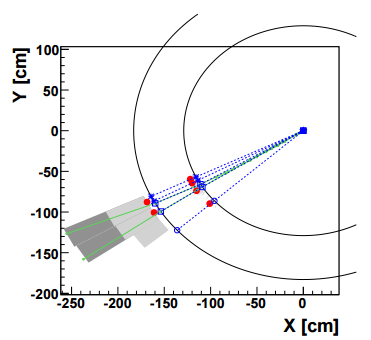
\includegraphics[width=0.6\textwidth]{Figures/PF.png}
\end{center}
\caption{The (x, y) view \cite{CMS-PAS-PFT-09-001}.}
\end{figure}

\begin{figure}
\begin{center}
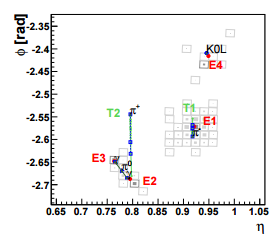
\includegraphics[width=0.7\textwidth]{Figures/PFECAL.png} \\
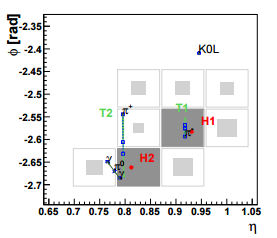
\includegraphics[width=0.7\textwidth]{Figures/PFHCAL.png} \\
\end{center}
%\caption{The ($\eta$, $\phi$) view on ECAL \cite{CMS-PAS-PFT-09-001}. 
\caption{The ($\eta$, $\phi$) view on HCAL \cite{CMS-PAS-PFT-09-001}.}
\end{figure}
   

\subsection{Electron reconstruction} \label{subsec-ElectronReconstruction}

For the $t\bar{t}+\gamma$ analysis it is imperative that the identification and energy-momentum requirements are measured extremely accurately as final state electrons, which are required in two of the three decay modes in the dilepton channel, can imitate a photon by passing the same selection, and therefore contaminating signal events. In order for electrons to be reconstructed with these strict requirements they are processed in a specific way.

The CMS ECAL and tracker systems are extremely accurate detectors, however reconstruction of energy deposits within the ECAL is still a complex task due to the density of material. As a charged particle traverses the detector volume, the energy lost due to interaction with the material is not negligible. Most charged particles are heavy enough such that the energy lost manifests in the form of multiple Coulomb scattering as the particle passes between material. However, in the case of electrons, the dominant process by which the energy is lost is due to Bremsstrahlung, the process by which photons are emitted upon passing through the electric and magnetic fields of a nucleus, such as the material in the detectors. 

Kalman fitters are a key tool used for the fitting of tracks in CMS due to their ability to incorporate noise amongst other inconsistencies,such as multiple scattering in track fitting, as Gaussian fluctuations. However, Bremsstrahlung radiation is non-Gaussian, and as a result electron tracks are poorly reconstructed with the standard Kalman filter fitting. To account for this, CMS provides a dedicated tool for the reconstruction of electrons using a Gaussian-sum filter (GSF) \cite{0954-3899-31-9-N01}. This method is implemented by calculating the trajectory of electrons using a `relaxed' Kalman filter, then re-fitted using a Gaussian-Sum Filter. The GSF method differs from the standard Kalman fitting method by computing uncertainties as the sum of multiple Gaussians rather than individual Gaussians. The downside to this method lies in the additional CPU time needed to process the events. 

The PF algorithm uses two different techniques of electron identification that are used as seeds when reconstructing electron \cite{CMS-PAS-PFT-10-003}. The first makes use of ECAL superclusters, extended clustering in $\phi$ due to Bremsstrahlung and photon conversions in the ECAL, as seeds and projects back from the centre of the supercluster to the innermost layer of the pixel detector, and is thus known as `ECAL-seeding'. It makes use of ECAL track properties, such as a narrow width in $\eta$ and a wide spread in the azimuthal angle, $\phi$. The energy deposits of the object and its associated Bremsstrahlung form a single supercluster, where the performance of this method lies the ability to correctly identify this. The method performs much more accurately in the high p$_T$ region of the electrons, such that there are much fewer potential track seeds and energy clusters in the ECAL are less likely to overlap with deposits from other objects, such as jets. This is especially true if the electron is part of a jet structure, and thus not isolated. Moreover, a high track multiplicity can complicate the backwards propagation from a supercluster and mimic the signal of another object.

The second, tracker-driven, method is much more suited for the efficient reconstruction of non-isolated and low p$_T$ electrons as they will most likely emit negligible amounts of Bremsstrahlung, and thus be fully reconstructed by extrapolating the tracks to superclusters. The cluster energy is then measured along with the track momentum, and if the ratio $E/p$ is close enough to unity then the track is selected. However, Bremsstrahlung is not always negligible and other track properties are used in the calculation. For example, the number of hits recorded in the inner tracker and the $\chi^2_{KF}$ of the Kalman filter fit are taken into account before refitting using a GSF, before being characterised by a multivariate estimation tool \cite{Roe2005577}. 

After both procedures have been performed the two collections of electron candidates are merged into one where a GSF is run in order to determine the final properties of the object. It is important for the GSF to be run at this stage in the process such that more hits can be included in the reconstruction, thus providing a more accurate description of the electron's energy and momentum lost by interacting with the detector material. Upon completion of the process, the GSF electrons are passed to the PF algorithm.

\subsection{Electron identification} \label{subsec-ElectronIdentification}

Electrons are identified in the ECAL and can be recognised by their distinct shower shape deposited within the calorimeter crystals. However, other objects such as charged hadrons, jets, and converted photons can have a very similar signature to an electron deposit and may be wrongly reconstructed as such. Therefore, in order to correctly reconstruct an electron candidate, we must implement further selection criteria. 

Individual physics analyses in CMS require different identification requirements tailored to personal needs, thus identification working points are initially required to be much looser than final cuts while still retaining a high efficiency of detecting electrons. When a further tight working point is implemented the efficiency for correctly selecting an electron increases. CMS uses various identification algorithms in order to correctly identify electrons: Simple cut-based ID, cuts in categories ID, particle flow ID, and MVA ID. Each of which are used in the analysis described in this thesis, and are described below.  

\begin{description}
	\item[Simple cut-based ID] Cut-based identification techniques, while not providing the greatest performance compared with other techniques, can be a useful tool in the understanding of the data and for making comparisons with MC.  Fewer variables from Table \ref{tab-ElectronMVAID} are used with this method, such as $H/E$, $\Delta \eta_{in}$ and $\Delta \phi_{in}$ between supercluster position and track direction at the vertex extrapolated to ECAL assuming no radiation, $\sigma_{i \eta i \eta}$ cluster and shape variables. \cite{CutBasedEleID}
	\item[Cuts in categories ID] is a more complex version of the simple cut-based identification techniques. It makes use of electrons originating from different sources, such as $Z$ and $W$ decays, while reducing the likelihood of wrongly selecting ``fake" electrons originating from photon conversions or jet mis-identifications, however the method has also been used to select electrons from alternative sources, such as the $J/\psi$. The problem of identifying electrons in CMS differs to that of other experiments due to the detector topology --- the large amount of material from the tracker directly in front of the ECAL and the high magnetic field make it difficult to efficiently reconstruct electrons. It has been found that many of the problems faced in the identification of electrons can be overcome by dividing the problem into categories. The most basic category sees the ECAL split into barrel and endcap regions due to the differences in topology in the two regions for both the inner tracker and ECAL. The second comes from the large amount of bremsstrahlung radiation in the tracker material, then using the measurement for $E/p$ to account for the poor reconstruction of the track. The final category divides electrons into high- and low-E$_T$ groups to correct for effects from the high magnetic field at high E$_T$.

	The cuts in categories method uses the same variables as the simple cut-based method with the addition of track conversion rejection (number of missing hits near beginning of track), and track isolations with tracker isolation ($\Delta R = 0.3$), ECAL Isolation (jurassic $\Delta R = 0.4$), HCAL Isolation ($\Delta R = 0.4$). The cuts are applied such that the signal to background ratio is optimised, where there are several levels of cut severity: \emph{VeryLoose, Loose, Medium, Tight, SuperTight, HyperTight (1-4)}. Each step of cut severity decreases the electron fake rate by roughly a factor of two for E$_T > 20$ GeV.  \cite{CutsInCategories} 
	\item[Particle Flow ID] is the loosest of all the electron identification techniques as it is a universal particle collection for all physics analyses. The method takes information from all subdetectors and combines it in order to create new observables to aid in the identification of electrons. These variables are shown in Table \ref{tab-ElectronMVAID} and are input into a multivariate analysis tool which then results in a discriminating value. The MVA is trained with respect to signal and background MC samples. \cite{PFElectronReconstruction}
	\item[MVA ID] is a multivariate analysis identification technique, and the most robust and common technique in physics analysis. It is used to identify electrons originating from W and Z bosons. The variables, show in Table \ref{tab-ElectronMVAID}, are used to produce a single discriminating value. The value is optimised by so called ``training" of the MVA in different selection categories.
\end{description}

\begin{center}
\begin{longtable}{|l|p{11cm}|}
\hline
	\textbf{Variable} & \textbf{Description} \\
\hline	
	\multicolumn{2}{|c|}{\emph{Track quality variables}}  \\
\hline
	p$_T$ & Transverse momentum of the GSF track \\
	$\eta$ & Pseudorapidity of the GSF track \\
	GSF $\sigma_{p_T}/p_T$ & Transverse momentum resolution of the GSF track \\
	\#hits$_{KF}$ & Number of reconstructed KF track hits \\
	$\chi^2_{GSF}$ and $\chi^2_{KF}$ & GSF and KF goodness-of-fits \\
\hline	
	\multicolumn{2}{|c|}{\emph{ECAL shower variables}} \\
\hline	
	$\sigma_{i \eta i \eta}$ & Cluster shape variable that gives a measure of the width of the cluster in $\eta$, using the distribution of energy in a $5 \time 5$ block of crystals around the seed crystal (the one with the highest energy) \cite{Baffioni:2006cd}: $\sigma^2_{i \eta i \eta} = \Sigma_{5 \times 5 crystals} (\eta_i \eta_{seed cluster})^2 E_i/E_{seed cluster}$ \\
	$\sigma^2_{i \phi i \phi}$ & Cluster shape in $\phi$ \\
	$\eta_{SC}(\phi_{SC})$ & Width of the super-cluster in $\eta (\phi)$ \\
	$1-E_{1 \times 5}/E_{5 \times 5}$ & $E_{1 \times 5}$ is the energy in the central $1 \times 5$ strip of the $5 \times 5$ electron cluster, and $E_{5 \times 5}$ is its total energy. \\
	$E_{3 \times 3}/E_{SC,raw}$ & Ratio of the energy in the preshower detector to the raw super-cluster energy (only in the endcap region). \\
\hline	
	\multicolumn{2}{|c|}{\emph{Longitudinal shower shape variables}} \\
\hline	
	$H/E$ & Ratio of the hadronic energy associated with the electron candidate to the super-cluster energy. The hadronic energy is found by summing the HCAL towers in a cone of radius $\Delta R = 0.15$, centred at the super-cluster position. \\
	$H/(H+E_{e})$ & Hadron fraction of the shower, where H is the energy of the hadron cluster linked to the GSF track.\\
\hline	
	\multicolumn{2}{|c|}{\emph{Track/super-cluster matching variables}}\\
\hline	
	$\Delta \eta_{in} \Delta \phi_{in}$ & Distance in $\eta (\phi)$ between the super-cluster position and the extrapolated track position \\
	$\Delta \eta_{vtx} \Delta \phi_{vtx}$ & Distance in $\eta (\phi)$ between the super-cluster position and the position of the GSF track at vertex \\
	$\left( E_{e} + \sum E_{\gamma} \right)/p_{in}$ & Ratio of the super-cluster energy to the inner track momentum \\
	$E_{e}/p_{out}$ & Ratio of the electron cluster energy to the outer track momentum \\
	$1/E_{SC} - 1/p_T$ & Difference between inverse super-cluster energy and inverse track momentum \\
\hline	
	\multicolumn{2}{|c|}{\emph{Bremsstrahlung variables}} \\
\hline	
	$f_{brem}$ & Measured bremsstrahlung fraction, defined as: $f_{brem} = (p_{in} - p_{out})/p_{in}$, where $p_{in}$ is the initial track momentum at the vertex and $p_{out}$ is the track momentum at the last hit. \\
	$\sum E_{\gamma}/(p_{in - p_{out}})$ & Ratio between the Bremsstrahlung photon energy as measured by ECAL and by the tracker \\
	$EarlyBrem$ & Flag of $(E_{e} + \Sigma E_{\gamma}) > p_{in}$ inequality, corresponding to an electron emitting an ``early" Bremsstrahlung photon, i.e. before it has crossed at least three tracker layers \\
	$LateBrem$ & Flag of $E_e > p_{out}$ inequality, corresponding to an electron emitting a ``late" Bremsstrahlung electron, when the ECAL clustering is not able to disentangle the overlapping electron and photon showers \\
\hline
\caption{Variables used in electron identification algorithms \cite{SergeyThesis}.}
\label{tab-ElectronMVAID}
\end{longtable} 
\end{center}


\subsection{Muon reconstruction} \label{subsec-MuonReconstruction}

Reconstructing muons efficiently was one of the major focuses in the design of the CMS experiment, as can be seen from the name. A muon has a lifetime of around $\tau \sim 2.2 \mus$, thus allowing them to travel a relatively large distance through the detector. Higher transverse momentum muons, $p_T > 20 \GeV$, are energetic enough to traverse the entire detector without feeling any effects from Coulomb scattering, while muons with a transverse momentum of $p_T < 5 \GeV$ are generally stopped within the detector volume and decay to an electron and two neutrinos via the electroweak force. Muons are also reconstructed using the particle flow algorithm (Section \ref{subsec-PFAlgorithm}), however there are subtle differences between the standard usage of the PF algorithm and PF for muon identification, as will be described in this section. In relation to a top quark analysis, muons are produced from the W boson produced from the decay of the top. As a result, the muon will be produced at a close proximity to the primary vertex, and also well isolated. 

In order to reconstruct muons, two types of tracks are used: tracks reconstructed from hits in the inner tracker (tracker hits), and in the muon system known as `standalone-muon' tracks. Reconstruction in the muon system begins with hits in either the DC or CSC which have been merged to create short track segments. The Kalman Filter technique is then used to combine the segments into full tracks, as described in Section \ref{subsec-ChargedParticleTracking}. We can then define muons in two ways \cite{1748-0221-7-10-P10002}: 

\begin{description}
	\item[Tracker Muons] are reconstructed such that every track found in the inner tracker with $p_T > 0.5 \GeV$ and $|p| > 2.5$ GeV is regarded as a muon candidate. The standalone-muon candidate is then extrapolated to the muon system, while taking into account factors such as the magnetic field, energy losses from traversing the detector volume, and uncertainties from multiple scattering. If the muon candidate satisfies both conditions of being in the tracker and extrapolated to the muon system, then we define the object as a muon. The method is also known as the `inside-out' method.
	\item[Global Muons] use the `outside-in' method to reconstruct muons, conversely to tracker muons. The method works by taking a standalone-muon reconstructed in the muon system and matching it with a tracker muon by propagating onto a common surface. A global fit is then performed with the properties of both muon candidates, thus giving a \emph{global muon}. 
\end{description}

The two techniques for muon reconstruction are used in conjunction with one another due to the efficiency for tagging muons at different $p_T$ thresholds. For the case of global muons, a muon with a higher transverse momentum ($p_T > 20 \GeV$) is more efficiently reconstruction due to the the tracking depositing energy in each of the muon chambers. Conversely, muons with a lower $p_T$ ($p_T < 5 \GeV$) are more efficiently reconstructed in the tracking system, requiring a single muon segment. For the $t\bar{t}+\gamma$ analysis, the requirement of one or two reasonably high $p_T$ muons means that it benefits from the use of both types of reconstruction method.

Once reconstructed, muons must undergo a series of quality checks in order to suppress punch through hadrons (hadrons that have a high enough energy to penetrate into the muon system from the HCAL). The following properties are used to select good muons for the $t\bar{t}+\gamma$ analysis.

\begin{itemize}
	\item The number of hit in the muon chamber in the global muon fit.
	\item The number of muon stations with muon segments.
	\item Normalised chi-squared ($\chi^2/N_{d.o.f}$) of the global muon fit
	\item The number of pixel detector hits.
	\item The number of hits in the tracker layers.
	\item Transverse impact parameter $d_{xy}$ (closest approach of the track to the primary vertex with respect to direction).
	\item longitudinal distance $d_z$ of the tracker track with respect to the primary vertex.
\end{itemize}

Muons can also be produced within jets. The PF algorithm reconstructs such particles and identifies them in order to reduce the fake rate of charged hadrons being misidentified. This technique is essential for the measurement of missing transverse energy. 

\section{Higher-level Object Reconstruction} \label{sec-HigherLevelObjects}

In this section we describe different techniques to reconstruct higher-level objects, such as jets and missing transverse energy, a process which happens post identification and reconstruction of objects. Higher-level objects must also be corrected for detector defects and other inconsistencies, which is also described.

\subsection{Jet reconstruction} \label{subsec-JetReconstruction}

We define a jet when a quark or gluon hadronises in an event, producing a narrow cone of collinear objects moving in the same direction. As described in Section \ref{chap-theory}, particles can not exist in an unbounded state as they carry a property known as colour and are confined within a hadron, and as a result they must fragment and form a hadron to be observed directly. Essentially, by reconstructing the sub-structures of jets, we are reverse-engineering the quantum-mechanical process of fragmentation and hadronisation. Therefore, if we wish to measure the initial energy and momentum, we must measure the combined properties of the reconstructed jet. 

Jets play an integral part in the identification of top quark events where, at the very least, there are two jets in the final state due to the hadronisation of b quarks. In the di-lepton channels the case is as described previously, however in the semi-leptonic and fully hadronic top decay channels, at least four jets are present in the final state. The jets originate from the hadronisation of the b quark, and W boson decaying to quarks, which in turn hadronise to create jets.  

In order to reconstruct jets, we first implement the PF algorithm in order to reconstruct single objects (muons, electrons, charged hadrons, neutral hadrons, and photons) before using clustering techniques to combine collinear particles to form jets. Various algorithms have been developed to compute the clustering of objects to form jets, such as the $k_t$ \cite{Ellis:1993tq}, Cambridge/Aachen \cite{Dokshitzer:1997in}, and SISCone \cite{Blazey:2000qt} jet clustering algorithms. However, the most widely used jet clustering algorithm is the anti-$k_t$ \cite{Cacciari:2008gp} algorithm, which is used by the majority of the CMS collaboration. There are two main requirements that reconstructed jets must comply with:

\begin{itemize}
	\item Collinear safe: should not be affected by collinear parton splitting.
	\item Infra-red safe: should not be affected by soft gluon emissions.
\end{itemize}

A low sensitivity to pileup and underlying events is also preferred in a jet clustering algorithm.

The anti-$k_t$ algorithm is particularly insensitive to pileup and underlying events. We start by defining a distance parameter, $d_{i,j}$, between entities (particles, pseudojets), and distance parameter $d_{iB}$ between entity i and the beam, B. The clustering method then begins by identifying the smallest of the distances, and if the smallest is $d_{i,j}$ then it recombines objects i and j, otherwise if the smallest distance is $d_{iB}$ then i is defined as a jet and is removed from the list of objects. The procedure is then repeated in an iterative fashion until there are no more objects to run over. The distances $d_{i,j}$ and $d_{iB}$ are defined as

\begin{equation}
d_{ij} = min\left(\frac{1}{k^2_{t,i}}, \frac{1}{k^2_{t,j}} \right) \cdot \frac{\Delta^2_{i,j}}{R^2}
\end{equation}
\begin{equation}
d_{iB} = \frac{1}{k^2_{t,i}}
\end{equation}

where $\Delta^2_{i,j} = (y_i - y_j)^2 + (\phi_i - \phi_j)^2$, $k_{t,i/j}$, $y_{i/j}$, and $\phi_{i/j}$ are the transverse momentum, rapidity, and azimuthal angle of each particle i and j, respectively. R is defined as the cone radius parameter. The anti-$k_t$ algorithm outputs conical jets such that their boundaries are less susceptible to soft radiation.

\subsection{Jet Identification} \label{subsec-JetIdentification}

PF jet identification is used in order to reduce the amount of noise and the rate of electrons misreconstructed as jets. In order to correctly reconstruct jets, a number of observables are used as listed below:

\begin{itemize}
	\item Number of particles in jet 
	\item Neutral hadron energy fraction (NHF) 
	\item Neutral electromagnetic energy fraction (NEF)
	\item Charged EM energy fraction (CEF)
	\item Charged hadron energy fraction (CHF)
	\item Charged hadron multiplicity (NCH)
\end{itemize}	

%%Talk about observables^^

\subsection{Jet energy corrections} \label{subsec-JEC}

Upon reconstruction of jets, we find that the jet energy is not the same when comparing MC generator and detector-level jets, even when reconstructed using the same algorithm. We find this to be due to the non-linear and non-uniformity of the CMS calorimetry, and a mis-modelling between MC simulation and performance of the detector including areas where we see a large amount of electronic noise and pileup. In order to correct for such discrepancies, we must apply corrections to the reconstructed jet energy - Jet Energy Corrections (JEC). The overall goal is to achieve a detector response that is linear and uniform in $\eta$, where we define the detector response as the average amount of signal per unit energy deposited.

CMS has developed a factorised three tier system in order to apply jet energy corrections \cite{1742-6596-404-1-012014}, such that each level corrects for a different effect. The corrections are then applied to the four-momentum of the jet. The three levels are described below.

\begin{itemize}
	\item \textbf{L1 Pile-up} corrects for any energy that does not originate from the hard-scattering event, including detector noise from electronics, and pile-up events.
	\item \textbf{L2 Relative Jet Correction} derives an $\eta$-dependent scale factor in order to flatten the detector response in order to account for the non-uniformity of the detector. MC and data-driven methods are used to calculate the relative correction scale factors using the dijet balance method. The corrections are measured using only the barrel region ($|\eta| < 1.3$) and in bins of $p_T$, such that they are completely uncorrelated with the L3 absolute correction described below. 
	\item \textbf{L3 Absolute Jet Correction} is a $p_T$-dependent correction used to correct back to particle level by applying absolute $p_T$ correction. This is derived using MC truth information, or data-driven di-leptonic decays from $Z/\gamma^*+Jets$ samples, with the aim of flattening the jet response in $p_T$. 
\end{itemize} 

There is also an extra component in the correction factor calculation that arises from discrepancies between MC modelling and data. We define this step as \textbf{L2L3 Residual} and is only applied to data \cite{1748-0221-6-11-P11002}. Higher order jet corrections, due to flavour-dependency, are also computed, however these are no included in this analysis. Uncertainties from each of the stages of correction are then convoluted into a single JEC systematic uncertainty included in the final result.  

\subsection{B-tagged Jets} \label{subsec-btaggedJets}

We define a b-tagged jet to be a jet that manifests from the hadronisation of a b-quark. The process of identification of b-jets, b-tagging, is an extremely important and vital part of physics analysis, and top quark physics in particular. As the top quark decays to a W boson and a b quark almost 100\% of the time, efficiently identifying b-jets significantly decreases the background contamination of our top quark signal process, and thus there is a strong need for b-tagging. Similar to non b-tagged jets, there are various algorithms that have developed by CMS that measure b-tagged jets \cite{Chatrchyan:2012jua}, with the most successful being the Combined Secondary Vertex (CSV) algorithm \cite{CSV}. This method is derived from the prolonged life-time of the b-quark ($10^{-12}s$), and the fact that they decay to up and charm quarks, transitions which are Cabibbo suppressed by the standard model and can be seen in the CKM matrix. A highly-relativistic b-quark will travel through the detector around $450 \mu m$, as a product of its long life-time, which is an observable length that can be measured by the pixel detector. This allows for a displaced secondary vertex to be used as a tool for the identification of b-jets, as seen in Figure \ref{fig-CSV}

\begin{figure} 
\begin{center}
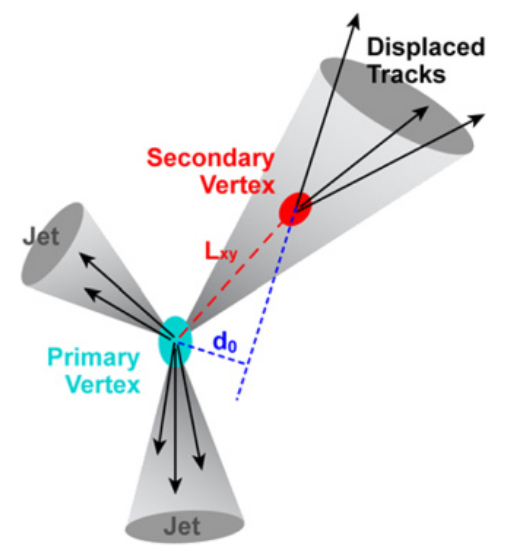
\includegraphics[width=0.5\textwidth]{Figures/CSV.png}
\end{center}
\caption{Schematic showing a displaced secondary vertex due to a b-quark decay from the primary vertex forming a b-jet. The impact parameter. $d_0$, measures the displacement with respect to the primary vertex along the z-axis, and $L_{xy}$ measures the displacement from the primary vertex in the transverse plane.}
\label{fig-CSV}
\end{figure}

B-tagged jets are particularly prominent due to their large mass, $4.18 \GeVcc$, and thus a large multiplicity of charged particles are produced during hadronisation carrying the majority of the jet energy. The most commonly used b-tagging algorithm is the Combined Secondary Vertex \cite{CSV} algorithm, which takes the following input parameters:

\begin{itemize}
	\item Track multiplicity in jet.
	\item Track multiplicity at secondary vertex.
	\item Secondary vertex category.
	\item The invariant mass of charged particles from the secondary vertex must not exceed $6.6 \GeVcc$ which would surpass the mass of the bottom quark when convoluted with its uncertainties.
	\item The ratio of the sum of the track energy at the secondary vertex to the sum of track energy of all tracks in jet.
	\item $\eta$ of the secondary vertex tracks with respect to the jet axis.
	\item The distance, $L_{xy}$, in the transverse plane between the primary and secondary vertex must be greater than $100 \mum$ and be less than $2.5 \cm$.
	\item Impact parameter significance ($L_{xy}/\sigma_{L_{xy}}$) of the first track, increasing the invariant mass above the threshold for charm production of $1.5 \GeV$.  
\end{itemize}

The algorithm begins by looking for a secondary vertex with the properties listed above. Using all particles in the jet, the algorithm uses a similar Kalman Filter \cite{VertexFitting} as for the reconstruction of primary vertices in order to reconstruct secondary vertices. If a secondary vertex is not found with this information, then a `pseudo-secondary vertex' is computed using information from the tracks that are were found to not be compatible with a primary vertex. The algorithm combines all of the information from the observables and calculates a discriminating value which is used to designate whether a jet is a `light jet' (a jet that manifests from a u,d, or s quark), a charmed jet (from a c quark), or a b-tagged jet. The CSV discriminator output can be seen in Figure \ref{fig-CSV}, showing the efficiency of correctly identifying a b-jet.

\begin{figure}
\begin{center}
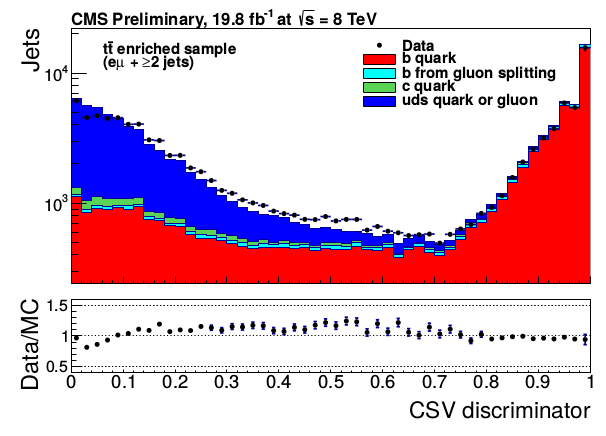
\includegraphics[width=0.8\textwidth]{Figures/CSVDiscriminator.png}
\end{center}
\caption{Logarithmic distribution of the partons as a function of the CSV b-tagging discriminant \cite{PhilThesis}.}
 \label{fig-CSVDiscriminator}
\end{figure}


\subsection{Reconstruction of Missing Transverse Energy} \label{subsec-METReco}

The conservation of momentum dictates that in an event, the sum of the $p_T$ of all final state particles (partons) must be equal to 0, as would be the case in a perfect detector. However, this is not the case within the CMS detector as particles, such as underlying events and proton remnants, are able to traverse the detector without being reconstructed. This introduces an imbalance in the measured transverse energy deposited in the detector, which we call the Missing Transverse Energy (MET). We can define the MET in an event to be:

\begin{equation}
E^{miss}_T = - \sum_i(p^2_x + p^2_y)^{1/2}
\end{equation}

where $p_x$ and $p_y$ are the transverse momenta of reconstructed particles (partons) in the x and y axes.

The reconstruction of MET is of particular importance when dealing with a measurement where the presence of weakly-interacting standard model particles are measured in the final state, such as neutrinos.  With respect to the $t\bar{t}+\gamma$ analysis, we expect a large amount of MET due to the presence of two neutrinos in the final state for each decay mode (excluding the $e\mu$ channel) of the di-lepton channel, as the W from the top quark will for decay to a lepton-neutrino pair $1/9th$ of the time. These channels, and other similar analysis, rely on the efficient reconstruction of MET in order to accurately measure certain processes, and any misidentification or poorly reconstructed particles add to the MET sum further reducing the accuracy of a measurement.  

Various methods on the reconstruction of MET in events have been conducted and are available \cite{1748-0221-6-09-P09001}. The current most accurate method for the measurement of the MET is by using the PF algorithm, and is used throughout this analysis. The PF algorithm calculates the value of the MET from the list of PF particles, thus producing a `raw' MET output which is systematically different from the final MET calculation. The `raw' MET value is calculated without taking into account the non-linearity of the calorimeters, noise from electronics, pile-up, along with any other effects. We, therefore, implement a set of corrections as described below.

\begin{description}
	\item[Type-0] corrects for the effects of pule-up on the MET.
	\item[Type-1] propagates the jet energy corrections into the MET (See Section \ref{subsec-JEC}). 
	\item[xy-shift] corrects for $\phi$ modulation in the MET.
\end{description}

The source of the $\phi$ modulation arises from misalignment of the detector relative to the beam, beam-spot displacement, an anisotropic detector response, and also broken or inactive cells within the calorimetry system. The correction for the shift in x-y is implemented in order to restore the spherical symmetry of events, and flatten the distribution in $\phi$, thus correcting the measured distribution to the true distribution. This analysis makes use of all correction types using PF calculated MET. 